
%% USEFUL LINKS:
%% -------------
%%
%% - UiO LaTeX guides:          https://www.mn.uio.no/ifi/tjenester/it/hjelp/latex/
%% - Mathematics:               https://en.wikibooks.org/wiki/LaTeX/Mathematics
%% - Physics:                   https://ctan.uib.no/macros/latex/contrib/physics/physics.pdf
%% - Basics of Tikz:            https://en.wikibooks.org/wiki/LaTeX/PGF/Tikz
%% - All the colors!            https://en.wikibooks.org/wiki/LaTeX/Colors
%% - How to make tables:        https://en.wikibooks.org/wiki/LaTeX/Tables
%% - Code listing styles:       https://en.wikibooks.org/wiki/LaTeX/Source_Code_Listings
%% - \includegraphics           https://en.wikibooks.org/wiki/LaTeX/Importing_Graphics
%% - Learn more about figures:  https://en.wikibooks.org/wiki/LaTeX/Floats,_Figures_and_Captions
%% - Automagic bibliography:    https://en.wikibooks.org/wiki/LaTeX/Bibliography_Management  (this one is kinda difficult the first time)
%%
%%                              (This document is of class "revtex4-1", the REVTeX Guide explains how the class works)
%%   REVTeX Guide:              http://www.physics.csbsju.edu/370/papers/Journal_Style_Manuals/auguide4-1.pdf
%%
%% COMPILING THE .pdf FILE IN THE LINUX IN THE TERMINAL
%% ----------------------------------------------------
%%
%% [terminal]$ pdflatex report_example.tex
%%
%% Run the command twice, always.
%%
%% When using references, footnotes, etc. you should run the following chain of commands:
%%
%% [terminal]$ pdflatex report_example.tex
%% [terminal]$ bibtex report_example
%% [terminal]$ pdflatex report_example.tex
%% [terminal]$ pdflatex report_example.tex
%%
%% This series of commands can of course be gathered into a single-line command:
%% [terminal]$ pdflatex report_example.tex && bibtex report_example.aux && pdflatex report_example.tex && pdflatex report_example.tex
%%
%% ----------------------------------------------------


\documentclass[english,notitlepage,reprint,nofootinbib]{revtex4-1}  % defines the basic parameters of the document
% For preview: skriv i terminal: latexmk -pdf -pvc filnavn
% If you want a single-column, remove "reprint"

% Allows special characters (including æøå)
\usepackage[utf8]{inputenc}
% \usepackage[english]{babel}

%% Note that you may need to download some of these packages manually, it depends on your setup.
%% I recommend downloading TeXMaker, because it includes a large library of the most common packages.

\usepackage{physics,amssymb}  % mathematical symbols (physics imports amsmath)
\include{amsmath}
\usepackage{graphicx}         % include graphics such as plots
\usepackage{xcolor}           % set colors
\usepackage{hyperref}         % automagic cross-referencing
\usepackage{listings}         % display code
\usepackage{subfigure}        % imports a lot of cool and useful figure commands
% \usepackage{float}
%\usepackage[section]{placeins}
\usepackage{algorithm}
\usepackage[noend]{algpseudocode}
\usepackage{subfigure}
\usepackage{tikz}
\usetikzlibrary{quantikz}
% defines the color of hyperref objects
% Blending two colors:  blue!80!black  =  80% blue and 20% black
\hypersetup{ % this is just my personal choice, feel free to change things
    colorlinks,
    linkcolor={red!50!black},
    citecolor={blue!50!black},
    urlcolor={blue!80!black}}


% ===========================================


\begin{document}
%\raggedbottom

\title{Numerical simulation of a Penning trap}  % self-explanatory
\author{Alessio Canclini, Filip von der Lippe} % self-explanatory
\date{\today}                             % self-explanatory
\noaffiliation                            % ignore this, but keep it.

%This is how we create an abstract section.
\begin{abstract}
    NB! ABSTRACT HERE
    %We provide an overview of how to structure a scientific report. For concreteness, we consider the example of writing a report about an implementation of the midpoint rule of integration. For each section of the report we briefly discuss what the purpose of the given section is. We also provide examples of how to properly include equations, tables, algorithms, figures and references.
\end{abstract}
\maketitle


% ===========================================
\section{Introduction}
The purpose of this report is to present the study of the effects of a Penning trap through numerical simulations. The Penning trap is a device used to store or "trap" charged particles
using static electric and magnetic fields as shown in figure \ref{fig:Penning_trap}. These particles can then be used for a variety of experiments. Examples of this are the ALPHA, AEgIS and BASE
experiments at CERN, these use Penning traps to control antimatter.
The electric field is generated by two end caps (a), at the top and bottom,
and a ring (b) (figure \ref{fig:Penning_trap} only shows the ring cross-section).
This electric field restricts the particles' movement in the $z$ direction and the additional homogenous magnetic field
hinders particles escaping in the $xy$-plane (radial direction) if it is strong enough. The magnetic field is set by
a cylinder magnet (c) (figure \ref{fig:Penning_trap} again only shows the ring cross-section).

Materials to construct a physical Penning trap are very costly, we will therefore
be using a numerical approach to simulate a Penning trap. To implement such a simulation
we will be working with a system of coupled non-linear differential equations. These are very
difficult and often impossible to solve analytically. %An example some readers might be familiar with are the famous
%Navier-Stokes equations, the solving of which would be rewarded with a million dollar prize.
In addition to the
material cost, the complexity of the equations therefore also motivates the use of numerical methods.

We will first explore the basic behavior of the Penning trap simulation and then look into some Penning trap physics. Expecting
the trap to be a system with complicated periodic particle motions, we will subject the trap to a time-dependent electromagnetic field
to look for possible resonance phenomena.


Section \ref{sec:methods} will describe the mathematical and physical background as well as concrete algorithms which in this case will be
implemented in C++, but can be written in any programming language.

In section \ref{sec:results} we present a selection of results form different simulations and an error analysis. This will include
simulations with a single particle, 2 particles and 100 random particles.

A detailed discussion of the algorithms' and results is presented in section \ref{sec:discussion},
followed by a summary and potential for further experiments in section \ref{sec:conclusion}.

\begin{figure}[H]
    \centering
    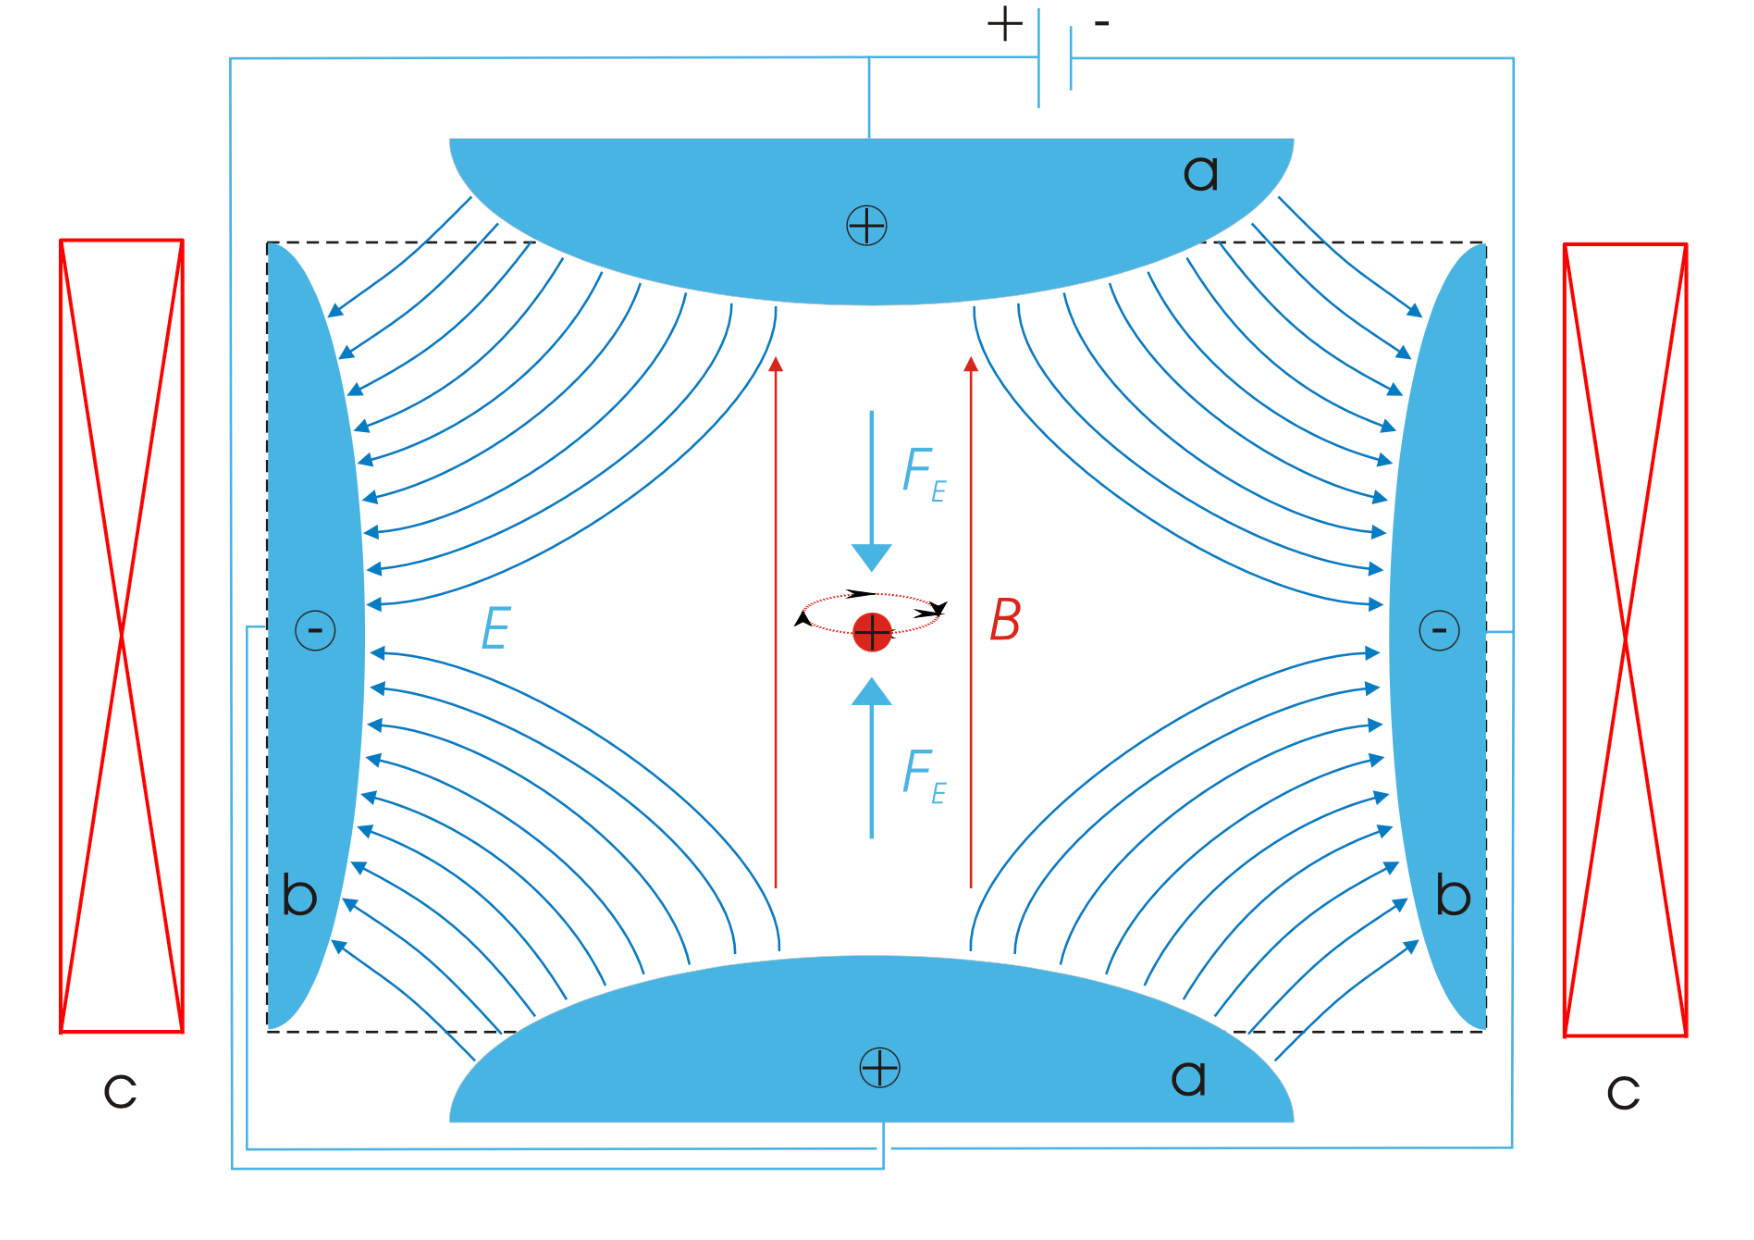
\includegraphics[width=.5\textwidth]{../figures/Penning_trap.pdf}
    \caption{This figure shows the idea of a Penning trap with a red positively charged particle in the center.
        Here blue lines represent the electric field generated by a quadrupole consisting of end caps (a) and a ring electrode (b).
        The red lines represent the magnetic field created by a surrounding cylinder magnet (c).
        Illustration by Arian Kriesch taken from Wikimedia Commons.}
    \label{fig:Penning_trap}
\end{figure}

% ===========================================
\section{Methods}\label{sec:methods}
The physical laws used to implement the Penning trap simulation will be from electrodynamics and classical mechanics, we will not take quantum aspects into account.
The following equations will be used:

\begin{equation}\label{eq:el_field}
    \textbf{E} = - \nabla V
\end{equation}
$\textbf{E}$ is the electric field and $V$ the electric potential.

\begin{equation}\label{eq:el_at_r}
    \textbf{E(r)} = k_e \sum_{j=1}^{n} q_j \frac{\textbf{r} - \textbf{r}_j}{|\textbf{r} - \textbf{r}_j|^3}
\end{equation}
$\textbf{E(r)}$ is the electric field at a point \textbf{r}. This is set up by point charges ${q_1,...,q_n}$ at points ${\textbf{r}_1,...,\textbf{r}_n}$. This comes from \textbf{Coulomb's law}, stating the magnitude of force between to point charges. $k_e \approx 8.988 \cdot 10^9 N m^2 C^{-2}$ is the Coulomb constant.

\begin{equation}\label{eq:lorentz}
    \textbf{F} = q\textbf{E} + q \textbf{v} \cross \textbf{B}
\end{equation}
This is the $\textbf{Lonretz force}$, the force $\textbf{F}$ on a particle
with charge $q$, an electric field \textbf{E}, magnetic field \textbf{B} and velocity of the particle \textbf{v}.

\begin{equation}\label{eq:N2L}
    m \ddot{\textbf{r}} = \sum_i \textbf{F}_i
\end{equation}
Eq. \ref{eq:N2L} is Newton's second law. Here $m$ is the mass of the particle and $\ddot{\textbf{r}} \equiv \frac{d^2 \textbf{r}}{dt^2}$ the acceleration.
Famously expressing that the sum of external forces equals mass times acceleration.
\begin{equation}\label{eq:el_potential}
    V(x,y,z) = \frac{V_0}{2d^2} (2z^2 - x^2 - y^2)
\end{equation}
For this experiment we will be considering an ideal Penning trap for which the electric field $\textbf{E}$ is given by the electric potential $V$.
Here $V_0$ is the potential applied to the electrodes. The trap will be approximated as a sphere where $d = \sqrt{z_0^2 + r_0^2 / 2}$ is the
$\textit{charachteristic dimension}$ representing the length scale (or radius of the sphere)
for the region between electrodes. Here $z_0$ is the distance from the center to the end caps (a) and $r_0$ is the distance from the center
to the surrounding ring (b).
\begin{equation}\label{eq:mag_field}
    \textbf{B} = B_0 \hat{e}_z = (0,0,B_0)
\end{equation}
$\textbf{B}$ is the homogenous magnetic field and is dictated by the field strength $B_0$. With $B_0 > 0$.

\subsection*{Equations for single particle motion}
Now starting from Newton's second law and using the equations above we can express the time evolution of a single particle's motion.
The sum of forces will be the Lonretz force. Putting eq. \ref{eq:lorentz} into eq. \ref{eq:N2L} leads to:
\begin{equation}\label{eq:N2L_lorentz}
    m \ddot{\textbf{r}} = q\textbf{E} + q \textbf{v} \cross \textbf{B}
\end{equation}
Here $\ddot{\textbf{r}} = (\ddot{x},\ddot{y},\ddot{z})$ and $\textbf{v} = (\dot{x},\dot{y},\dot{z})$. Putting eq. \ref{eq:el_potential} into eq. \ref{eq:el_field} gives us:
\begin{equation}\label{eq:el_calculated}
    \textbf{E} = \left( x \frac{v_0}{d^2}, y \frac{v_0}{d^2}, -2z \frac{v_0}{d^2} \right)
\end{equation}
Now looking at $q \textbf{v} \cross \textbf{B}$ we have:
\begin{equation}\label{eq:cross_calculated}
    (q \dot{x},q \dot{y},q \dot{z}) \cross (0, 0, B_0) = (B_0 q \dot{y}, -B_0 q \dot{x}, 0)
\end{equation}
Finally substituting for $\textbf{E}$ and $q \textbf{v} \cross \textbf{B}$ in eq. \ref{eq:N2L_lorentz} results in:
\begin{equation*}
    m \begin{pmatrix}
        \ddot{x} \\ \\ \ddot{y} \\ \\ \ddot{z}
    \end{pmatrix}
    = \begin{pmatrix}
        q x \frac{v_0}{d^2} \\ \\ q y \frac{v_0}{d^2} \\ \\ -2 q z \frac{v_0}{d^2}
    \end{pmatrix}
    + \begin{pmatrix}
        B_0 q \dot{y} \\ \\ -B_0 q \dot{x} \\ \\ 0
    \end{pmatrix}
\end{equation*}
Rewriting this as a set of equations leaves us with:
\begin{align}
    \ddot{x} - w_0 \dot{y} - \frac{1}{2} & w_z^2 x = 0 \label{eq:a_x} \\
    \ddot{y} + w_0 \dot{x} - \frac{1}{2} & w_z^2 y = 0 \label{eq:a_y} \\
    \ddot{z} + w_z^2                     & z = 0 \label{eq:a_z}
\end{align}
Where $w_0 = \frac{qB_0}{m}$ and $w_z^2 = \frac{2qV_0}{md^2}$. Taking a closer look at eq. \ref{eq:a_z} we see that the general solution is:
\begin{equation}
    z = A \cos(w_z t) + B \sin(w_z t)
\end{equation} \label{eq:z_general}
eq. \ref{eq:a_x} and \ref{eq:a_y} are coupled, thus introducing a challenge. This can be resolved by introducing a complex function $f(t) = x(t) + iy(t)$ and rewriting them as a single differential equation. By introducing the complex function we have:
\begin{align}
    f(t) = x(t) + iy(t)                   \\
    \dot{f}(t) = \dot{x}(t) + i\dot{y}(t) \\
    \ddot{f}(t) = \ddot{x}(t) + i\ddot{y}(t)
\end{align}
Now multiplying eq. \ref{eq:a_y} by $i$ gives:
\begin{equation}
    i\ddot{y} + iw_0 \dot{x} - i\frac{1}{2} w_z^2 y = 0 \label{eq:a_iy}
\end{equation}
eq. \ref{eq:a_x} and \ref{eq:a_iy} can then be summed:
\begin{equation}
    \ddot{x}+ i\ddot{y} - w_0 \dot{y} + iw_0 \dot{x} - \frac{1}{2} w_z^2 x - i\frac{1}{2} w_z^2 y= 0
\end{equation}
Finally, substituting for $f(t)$, $\dot{f}(t)$ and $\ddot{f}(t)$ shows that eq. \ref{eq:a_x} and \ref{eq:a_y} can be rewritten as a single differential equation for $f$:
\begin{equation}
    \ddot{f} + i w_0 \dot{f} - \frac{1}{2} w_z^2 f = 0 \label{eq:single_diff}
\end{equation}

The general solution to eq. \ref{eq:single_diff} is:
\begin{equation}
    f(t) = A_+ e^{-i(w_+ t + \phi_+)} + A_- e^{-i(w_- t + \phi_-)} \label{eq:general_sol_f}
\end{equation}
where the amplitudes $A_+$ and $A_-$ are positive, $\phi_+$ and $\phi_-$ are constant phases, and
\begin{equation}
    w_\pm = \frac{w_0 \pm \sqrt{w_0^2 - 2 w_z^2}}{2}
\end{equation}
To obtain a bounded solution for the radial movement ($xy$-plane) of the particle we need to introduce some constraints on $w_0$ and $w_z$. In other words we will introduce some constraints that will ensure that $|f(t)| < \infty$ as $t \rightarrow \infty$.

Studying eq. \ref{eq:general_sol_f} one notices that $|f(t)| \rightarrow \infty$ only if $w_\pm$ is complex. To avoid this, we introduce the limitation $w_0^2 - 2 w_z^2 \geq 0$, avoiding any negative values inside the square root and consequently limiting the result to real numbers. Rearranging this and remembering that $w_0 = \frac{qB_0}{m}$ and $w_z^2 = \frac{2qV_0}{md^2}$ leaves us with:
\begin{equation}
    \frac{q}{m} \geq \frac{4 V_0}{B_0^2 d^2}
\end{equation}
A constraint, that if satisfied, keeps the particle within the Penning trap.

\subsection*{Upper and lower bounds}
Now to express the upper and lower bounds of the particles' distance from the origin in the $xy$-plane
we start with eq. \ref{eq:general_sol_f}. Through Taylor expansion of $e^{ix}$ we arrive at Euler's formula:
\begin{equation*}
    e^{ix} = \cos(x) + i \sin(x)
\end{equation*}
Introducing $u =  w_+ t + \phi_+$ and $v = w_- t + \phi_-$, and using
Euler's formula, eq. \ref{eq:general_sol_f} can be rewritten as:
\begin{equation*}
    f(t) = A_+\left(\cos(u) - i \sin(u) \right) + A_-\left(\cos(v) - i \sin(v) \right)
\end{equation*}
The physical coordinates can then be found as $x(t) = \Re f(t)$ and  $y(t) = \Im f(t)$. Giving us:
\begin{align*}
    x(t) & = A_+ \cos(u) + A_- \cos(v)  \\
    y(t) & = -A_+ \sin(u) - A_- \sin(v)
\end{align*}
Since our $xy$-plane is a circle, the particle's distance from the origin can be expressed as the radius $R = \sqrt{x^2 + y^2}$.
Substituting for $x$ and $y$ we have:
\begin{align*}
    R = & [ (A_+ \cos(u) + A_- \cos(v))^2 \\ &+ (-A_+ \sin(u) - A_- \sin(v))^2 ]^{1/2}
\end{align*}
After expanding and rearranging we have:
\begin{align*}
    R = & [A_+^2(\cos^2(u) + \sin^2(u)) + A_-^2(\cos^2(v) + \sin^2(v)) \\ &+ 2 A_+ A_- (cos(u)\cos(v) + \sin(u)\sin(v))]^{1/2}
\end{align*}
Recognizing that $cos^2(u) + \sin^2(u) = 1$ and $cos(u)\cos(v) + \sin(u)\sin(v) = \cos(u-v)$ this can be simplified to:
\begin{align*}
    R = \sqrt{A_+^2 + A_-^2 + 2 A_+ A_- \cos(u-v)}
\end{align*}
We know that $\cos$ is a function with an upper bound of $1$ and lower bound of $-1$.
The bounds for $R$ are consequently:
\begin{align*}
    R_+ & = \sqrt{A_+^2 +2A_+ A_- + A_-^2} = A_+ + A_-   \\
    R_- & = \sqrt{A_+^2 -2A_+ A_- + A_-^2} = |A_+ - A_-|
\end{align*}


\subsection*{Numbers and units}
The following units will be used for all simulation experiments:
\begin{itemize}
    \item Length: micrometer $(\mu \text{m})$
    \item Time: microseconds $(\mu \text{s})$
    \item Mass: atomic mass unit (u)
    \item Charge: the elementary charge (e)
\end{itemize}
With these units we end up with a Coulomb constant equal to:
\begin{itemize}
    \item $k_e = 1.38935333 \cross 10^5 \frac{\text{u} (\mu \text{m})^3}{(\mu \text{s})^2(\text{e})^2}$
\end{itemize}
SI units for Tesla (magnetic field strength) and Volt (electric potential) become:
\begin{itemize}
    \item $T = 9.64852558 \cross 10^1 \frac{\text{u}}{(\mu \text{s})\text{e}}$
    \item $V = 9.64852558 \cross 10^7 \frac{\text{u} (\mu \text{m})^2}{(\mu \text{s})^2 \text{e}}$
\end{itemize}
With these units the default penning trap configuration will be:
\begin{itemize}
    \item $B_0 = 1.00 \text{ T} = 9.65 \cross 10^1 \frac{\text{u}}{(\mu \text{s})\text{e}}$
    \item $V_0 = 25.0 \text{ mV} = 2.41 \cross 10^6 \frac{\text{u} (\mu \text{m})^2}{(\mu \text{s})^2 \text{e}}$
    \item $d = 500 \mu \text{m}$
\end{itemize}

\subsection*{Particles}
Our charged particles will be singly-charged Calcium ions $(Ca^+)$ with a mass of $40.077$u.
\begin{itemize}
    \item Particle 1:
          \subitem $(x_0,y_0,z_0) = (20, 0, 20) \mu \text{m}$
          \subitem $(v_{x,0}, v_{y,0}, v_{z,0}) = (0, 25, 0) \mu \text{m} / \mu \text{s}$
    \item Particle 2:
          \subitem $(x_0,y_0,z_0) = (25, 25, 0) \mu \text{m}$
          \subitem $(v_{x,0}, v_{y,0}, v_{z,0}) = (0, 40, 5) \mu \text{m} / \mu \text{s}$
\end{itemize}
Simulations with one particle will use initial conditions for Particle 1 whilst simulations with two particles will use both Particle 1 and Particle 2.
For further simulations with 100 particles, Armadillo's \texttt{vec::randu()} function will be used to generate random initial
positions and velocities for each particle.

\subsection*{Specific analytical solution}
To test the numerical solutions and for error analysis an analytical solution for
Particle 1 is used. For these initial condition the specific $z(t)$ solution for
eq. \ref{eq:z_general} becomes:
\begin{equation*}
    z(t) = z_0 \cos(\omega_z t)
\end{equation*}
The specific solution for motion in the $xy$-plane, $f(t)$ is given by eq. \ref{eq:general_sol_f}
with
\begin{align*}
    A_+ = \frac{v_0 + \omega_- x_0}{\omega_- - \omega_+}&, \quad A_- = -\frac{v_0 + \omega_+- x_0}{\omega_- - \omega_+} \\
    \phi_+ = 0&, \quad \phi_- = 0
\end{align*}


\subsection*{Equations for multiple particle motion}
For all simulations with more than one particle when particle interaction is taken into account,
the equations of motion will be coupled because of the Coulomb force between two point charges.
Our numerical algorithms will therefore be solving the following equations:
\begin{align}
    \ddot{x}_i - w_{0,i} \dot{y}_i - \frac{1}{2} & w_{z,i}^2 x_i - k_e \frac{q_i}{m_i} \sum_{j\neq i}^{n} q_j \frac{x_i - x_j}{|\textbf{r}_i - \textbf{r}_j|^3} = 0 \label{eq:a_x_coupled} \\
    \ddot{y}_i + w_{0,i} \dot{x}_i - \frac{1}{2} & w_{z,i}^2 y_i - k_e \frac{q_i}{m_i} \sum_{j\neq i}^{n} q_j \frac{y_i - y_j}{|\textbf{r}_i - \textbf{r}_j|^3} = 0 \label{eq:a_y_coupled} \\
    \ddot{z}_i + w_{z,i}^2                       & z_i - k_e \frac{q_i}{m_i} \sum_{j\neq i}^{n} q_j \frac{z_i - z_j}{|\textbf{r}_i - \textbf{r}_j|^3} = 0 \label{eq:a_z_coupled}
\end{align}
Here the summation term is the Coulomb force and $i$ and $j$ are particle indices for $n$ particles
with charges $\{q_1,...,q_n\}$ and masses $\{m_1,..,m_n\}$.
% ===========================================
\subsection*{The algorithms}
To evolve our Penning trap system in time the following algorithms will be implemented to solve our particles' equations of motion.
Consider the forward difference approximation for the first derivative based on Taylor expansion:
\begin{equation}
    y_n' = \frac{y_{n+1}  - y_n}{h}, \quad h = t_{t-1} -t_n
\end{equation}
Rearranging this results in the forward Euler method which has a local error of $\mathcal{O}(h^2)$ and global error of $\mathcal{O}(h)$,
making it only first order accurate. The method is easy to implement and will be used for comparisons
and checking of the main algorithm.
%
% The algorithm for the midpoint rule is summarized in algorithm~\ref{algo:midpointrule}. The basic idea behind the algorithm is to divide the integration range into to $n$ small subintervals of length $h$, and on each such subinterval approximate the function $f(x)$ by a constant function. The value for this constant function is taken to be the value of $f(x)$ evaluated at the midpoint of the given subinterval --- hence the name of the method.
% %
\begin{figure}[H]
    % NOTE: We only need \begin{figure} ... \end{figure} here because of a compatability issue between the 'revtex4-1' document class and the 'algorithm' environment.
    \begin{algorithm}[H]
        \caption{Forward Euler method}
        \label{algo:EUL}
        \begin{algorithmic}
            \Procedure{Forward Euler}{$y_0, h$}
            \State $y' = f(t_i,y_i)$        \Comment{Single fist-order diff. eq.}
            \State $n = 1 / h$ \Comment{Compute number of steps}
            \\
            \For{$i = 0, 1, 2, \ldots, n$}
            \State $y_{i+1} = y_i + h f(t_i, y_i)$  \Comment{Value at next time step}
            \EndFor
            \EndProcedure
        \end{algorithmic}
    \end{algorithm}
\end{figure}

Similarly to the forward Euler, Runge-Kutta fourth order (RK4) is based on Taylor expansion, but by adding several intermediate
steps to the computation of $y_{i+1}$ it generally yields better solutions for ODEs. RK4 has a local error of $\mathcal{O}(h^5)$
and global error of $\mathcal{O}(h^4)$. (REF COMPENDIUM HERE)

\begin{figure}[H]
    % NOTE: We only need \begin{figure} ... \end{figure} here because of a compatability issue between the 'revtex4-1' document class and the 'algorithm' environment.
    \begin{algorithm}[H]
        \caption{Runge-Kutta fourth order method}
        \label{algo:RK4}
        \begin{algorithmic}
            \Procedure{Runge-Kutta fourth order}{$y_0, h$}
            \State $y' = f(t_i,y_i)$        \Comment{Single fist-order diff. eq.}
            \State $n = 1 / h$ \Comment{Compute number of steps}
            \\
            \For{$i = 0, 1, 2, \ldots, n$}
            \State $k_1 = hf(t_i,y_i)$  \Comment{Intermediate step 1}
            \State $k_2 = hf(t_i + h/2, y_i +k_1/2)$  \Comment{Intermediate step 2}
            \State $k_3 = hf(t_i + h/2, y_i + k_2/2)$ \Comment{Intermediate step 3}
            \State $k_4 = hf(t_i + h, y_i + k_3)$ \Comment{Intermediate step 4}
            \State $y_{i+1} = y_i + \frac{1}{6}(k_1 + 2k_2 + 2k_3 + k_4)$ \Comment{Final algorithm}
            \EndFor
            \EndProcedure
        \end{algorithmic}
    \end{algorithm}
\end{figure}

The RK4 scheme will be our main method as this is a ``gold standard'' in numerical analysis.
Early tests with one single particle will be confirmed by an analytical solution, but for comparison of more complex
scenarios the simple forward Euler scheme will also be implemented.

The Penning trap with time evolving algorithms will be implemented in an object-oriented C++ code, the plots are generated using Python.

\subsection*{Resonance experiments}
We will be subjecting the Penning trap to a time-dependent electromagnetic field by adding a time-dependent perturbation
to the electric potential with a constant amplitude $f$ and angular frequency $\omega_V$. For resonance experiments the
following replacement will be made:
\begin{equation}
    V_0 \rightarrow V_0 (1 + f \cos(\omega_V t) )
\end{equation}
The simulation is run for 500 $\mu s$ for amplitudes $ f = 0.1, 0.4, 0.7$ and frequencies $\omega_V \in (0.2,2.5)$. The frequency
range is initially explored with a step size of $0.2$ MHz disregarding Coulomb interactions. An area of interest (in this case $\omega_V \in (2.05,2.35)$)
is then
looked at closely with smaller step sizes of 0.001 MHz once with Coulomb interactions and once without.
% \textit{As demonstrated in algorithm~\ref{algo:midpointrule}, it is conventional to present algorithms in a way that is independent of any specific programming language. This ensures that it is the logic behind the algorithm that remains in focus, rather than the syntax of a particular programming language. In algorithm~\ref{algo:midpointrule} we have also demonstrated a common notation: The right-to-left arrow ($\leftarrow$) means that we assign the value of everything on the right to the variable on the left. This is nothing but how the ``='' symbol functions in most programming languages, but the arrow notation makes it clear that we are in fact assigning a value, rather than stating that two things are equal.}

\subsection*{Error analysis}
To check the validity of our methods and gauge how realistic our Penning trap simulations are, we perform an error analysis of the
numerical methods implemented. This is done by considering the simple case of a single particle, making it easy to compare the numerical
to analytic results. The simulation with Particle 1 is run over 50 $\mu$s. This is done for four different step sizes $h_k = 50 / n_k \mu$s.
The chosen step sizes are for $n_1 = 4000, n_2 = 8000, n_3 = 16000, n_4 = 32000$. For each step size the relative error of $\textbf{r}_i$
for each time step $t_i$ is calculated for both algorithms.
Additionally, these results are used to calculate the error convergence rate in both cases.
% % ===========================================
\section{Results}\label{sec:results}
First we test our Penning trap's behavior for a single particle to see if it produces the expected motion in this simple case.
All three solutions have been plotted in figure \ref{fig:compare_analytic_tz} for $N=10000$ steps to examine weather the numerical and analytic results agree.
%single particle
\begin{figure}[H]
    \centering
    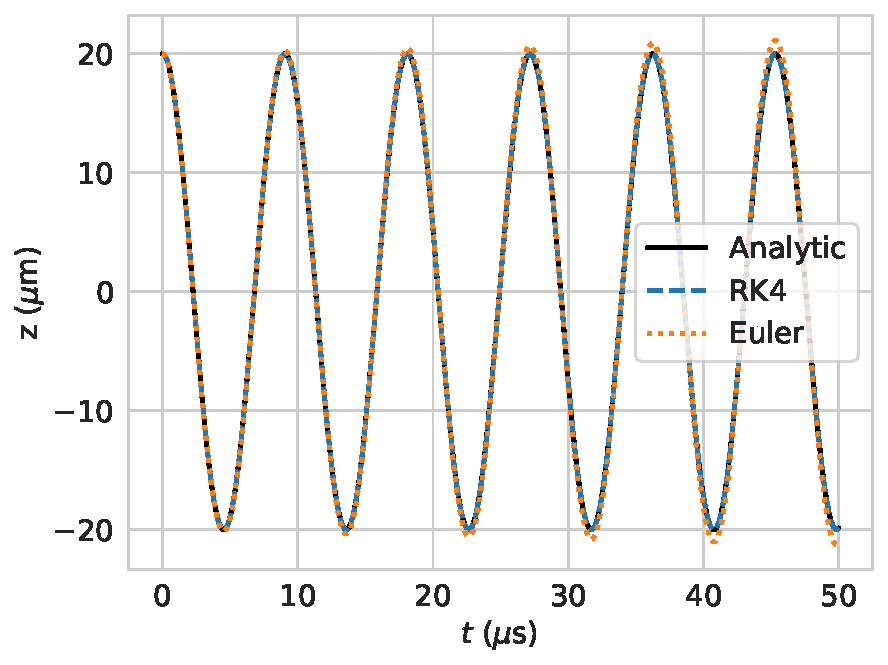
\includegraphics[width=.5\textwidth]{../figures/compare_analytic_t_axis_2_N10000.pdf}
    \caption{Here we see the vertical path of a single particle over 50 $\mu s$ for $N=10000$. The analytic, Euler and RK4 solutions are shown.}
    \label{fig:compare_analytic_tz}
\end{figure}
Figure \ref{fig:compare_analytic_tz} shows that both the forward Euler and RK4 method show the same
$z$ motion as the analytic solution for a single particle. The particle oscillates vertically but over time we notice a growing error for the Euler method, While RK4 seems to agree well with the analytic solution.

We again compare the three solutions but now using a smaller time step of $n=5000$.
\begin{figure}[H]
    \centering
    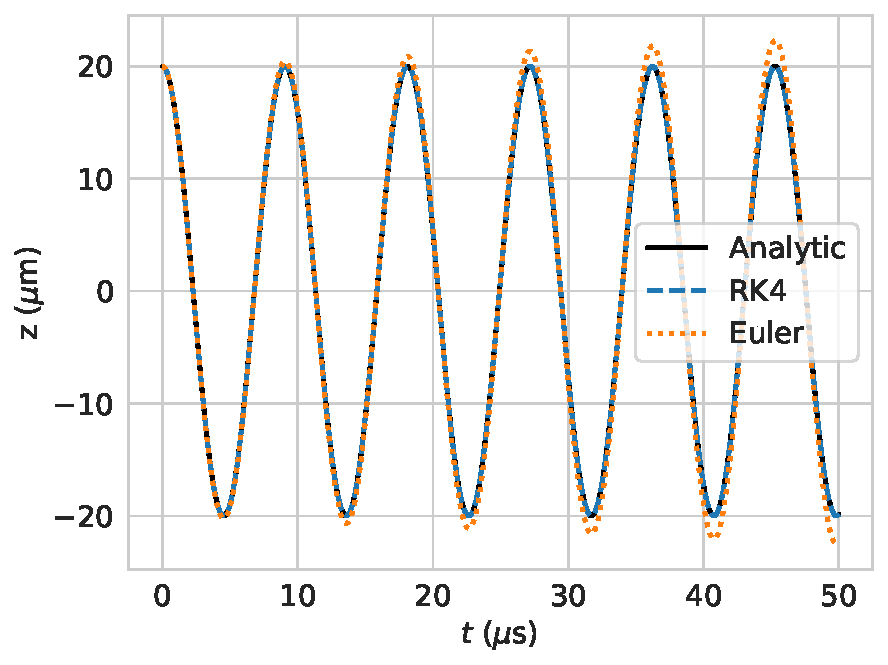
\includegraphics[width=.5\textwidth]{../figures/compare_analytic_t_axis_2_N5000.pdf}
    \caption{Here we see the vertical path of a single particle over 50 $\mu s$ for $N=5000$. The analytic, Euler and RK4 solutions are shown.}
    \label{fig:compare_analytic_tz_5000}
\end{figure}


\begin{figure}[H]
    \centering
    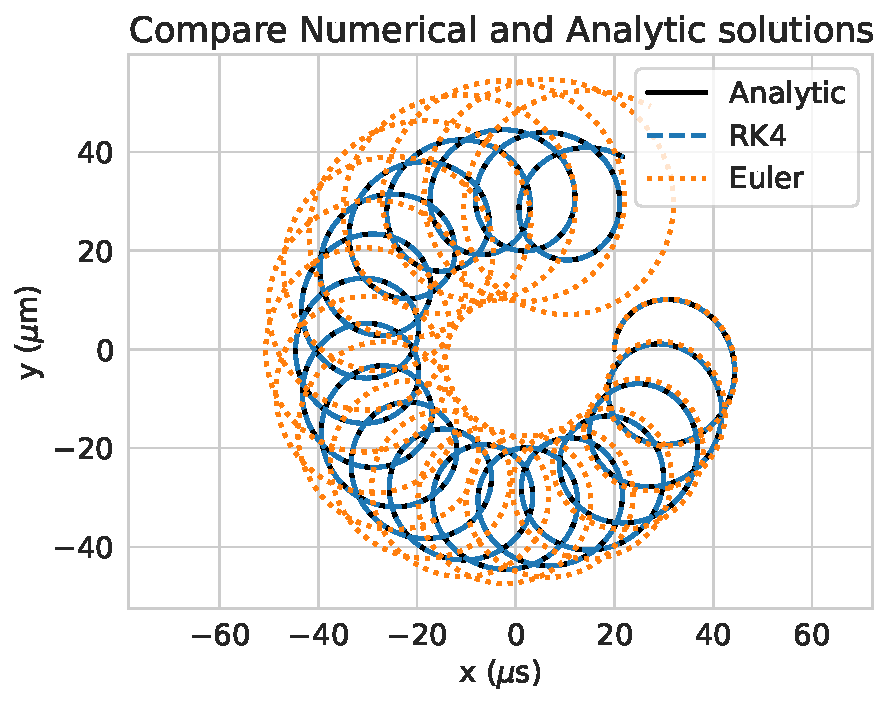
\includegraphics[width=.5\textwidth]{../figures/compare_analytic_axis_0_1_N10000.pdf}
    \caption{Horizontal motion of a single particle over 50 $\mu s$ for $N=10000$. The analytic, Euler and RK4 solutions are shown.}
    \label{fig:compare_analytic_axis_0_1_N10000}
\end{figure}
Figure \ref{fig:compare_analytic_axis_0_1_N10000} displays that the numerical methods perform as similarly for all spatial axes of the simulation.
\begin{figure}[H]
    \centering
    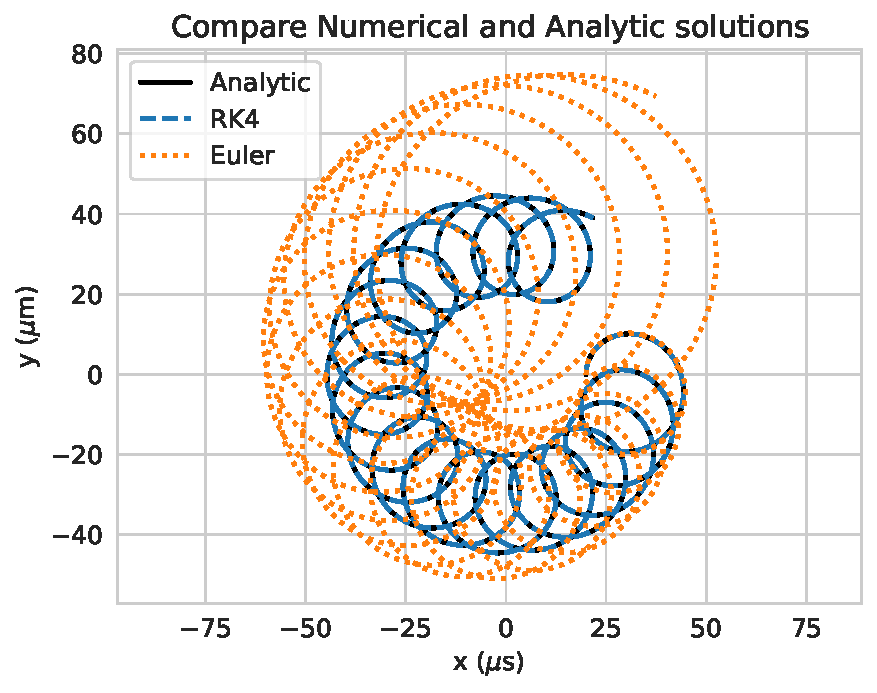
\includegraphics[width=.5\textwidth]{../figures/compare_analytic_axis_0_1_N5000.pdf}
    \caption{Horizontal motion of a single particle over 50 $\mu s$ for $N=5000$. The analytic, Euler and RK4 solutions are shown.}
    \label{fig:compare_analytic_axis_0_1_N5000}
\end{figure}
Above in figure \ref{fig:compare_analytic_tz_5000} and \ref{fig:compare_analytic_axis_0_1_N5000} we see a growing error for Euler while RK4 still agrees well with the analytic solution.
We also notice that a change in number of timesteps from $N=10000$ to $N=5000$ impacts the performence of the Euler method, while RK4 keeps its accuracy indicating the superiority of this method.
All this means that we now especially can trust the RK4 method but also Euler while keeping the timestep $h=T/N$ low.

%z motion over 500 , RK4 vs analytic
\begin{figure}[H]
    \centering
    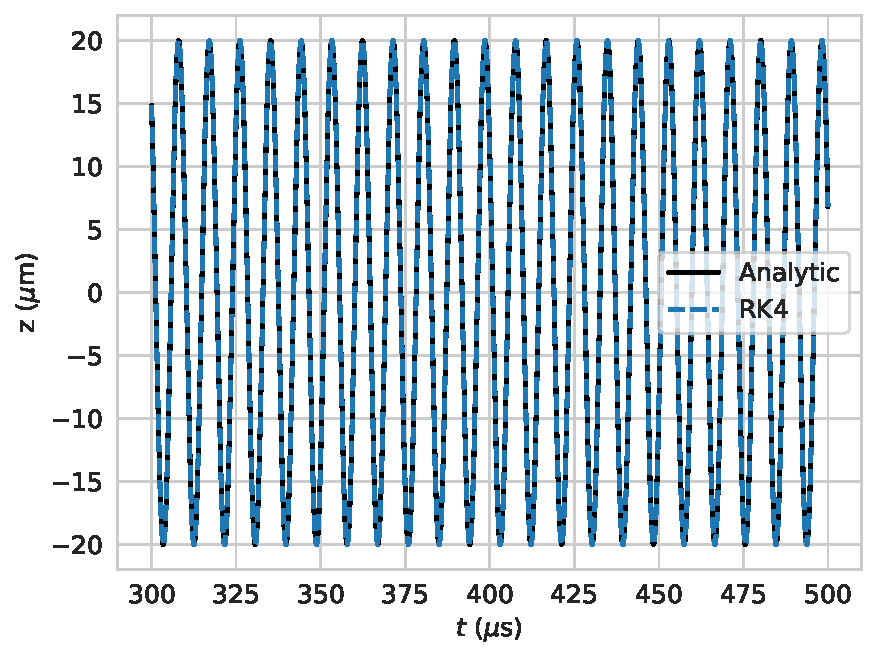
\includegraphics[width=.5\textwidth]{../figures/analytic_RK4_t_axis_2_N5000.pdf}
    \caption{Vertical motion of a single particle over 500 $\mu s$ for $N=5000$. The analytic and RK4 solutions are shown.}
    \label{fig:analytic_RK4_t_axis_2_N5000}
\end{figure}

Figure \ref{fig:analytic_RK4_t_axis_2_N5000} shows that the RK4 method agrees with the analytic solution even for a longer time period of 500 $\mu$s
Based on this we continue using $N=5000$ time steps and the RK4 method to plot the motion of Particle 1 and Particle 2 in the $xy$-plane when they do not interact.
That is, disregarding the Coulomb force.
%two particles
\begin{figure}[H]
    \centering
    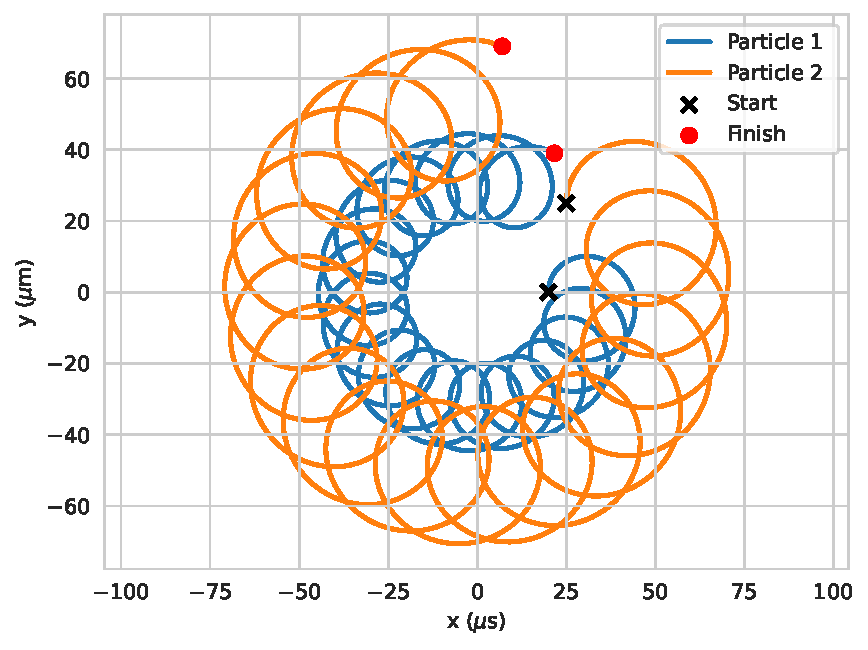
\includegraphics[width=.5\textwidth]{../figures/2p_N5000_RK4_xy.pdf}
    \caption{The horizontal ($xy$-plane) path of two particles without interaction for for $N = 5000$.}
    \label{fig:RK4_2_xy_no_interaction_xy}
\end{figure}
In figure \ref{fig:RK4_2_xy_no_interaction_xy}
The paths have a very similar spiraling shape both resulting circular patterns around the origin.

We continue with the same parameters and particles but now adding the Coloumb force as seen below in figure \ref{fig:RK4_2_xy_with_interaction_xy}.

\begin{figure}[H]
    \centering
    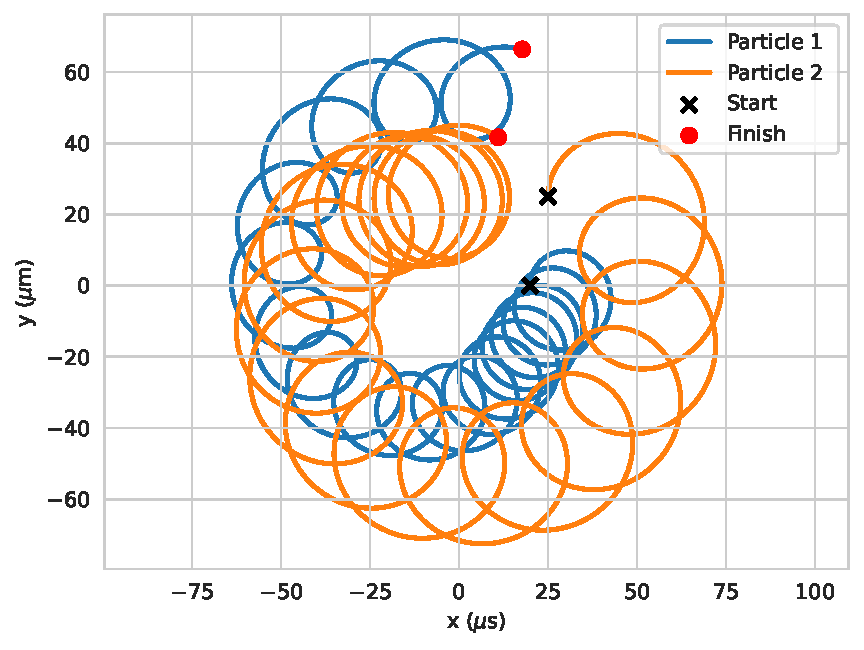
\includegraphics[width=.5\textwidth]{../figures/2p_N5000_RK4_xy_interaction.pdf}
    \caption{The horizontal ($xy$-plane) path of two particles with interaction for $N = 5000$.}
    \label{fig:RK4_2_xy_with_interaction_xy}
\end{figure}

In figure \ref{fig:RK4_2_xy_with_interaction_xy} we see a similar motion as in figure \ref{fig:RK4_2_xy_no_interaction_xy}. We notice that the paths, although still spiraling, are not as circular as a result of the added Coloumb force.


% Phase spaces xy
\begin{figure}[H]
    \centering
    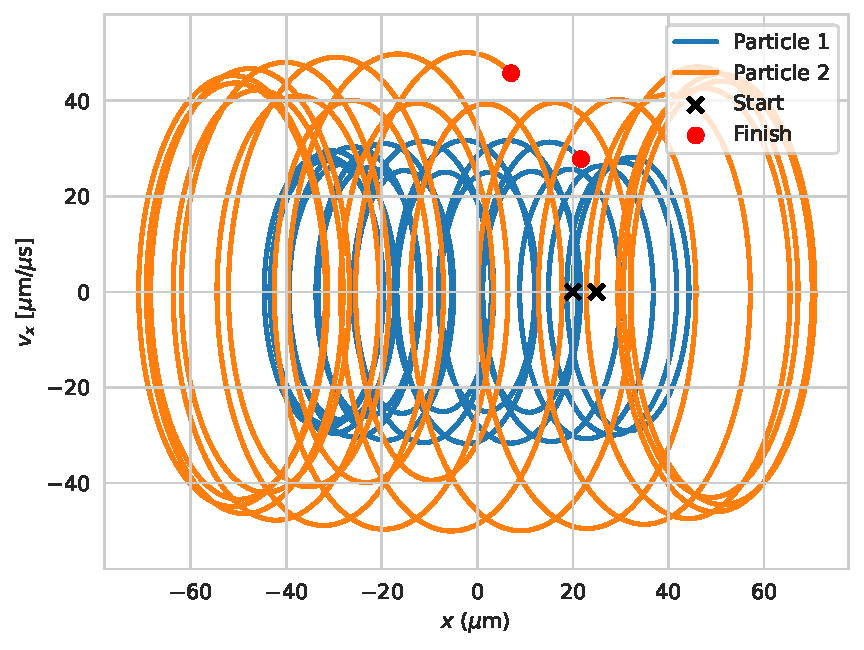
\includegraphics[width=.5\textwidth]{../figures/phase_space_x_RK4_N5000.pdf}
    \caption{The phase space $(x, v_x)$ of two particles without interaction for $N = 5000$.}
    \label{fig:RK4_2_x_phasespace_no_interaction_phasespace_xy}
\end{figure}

\begin{figure}[H]
    \centering
    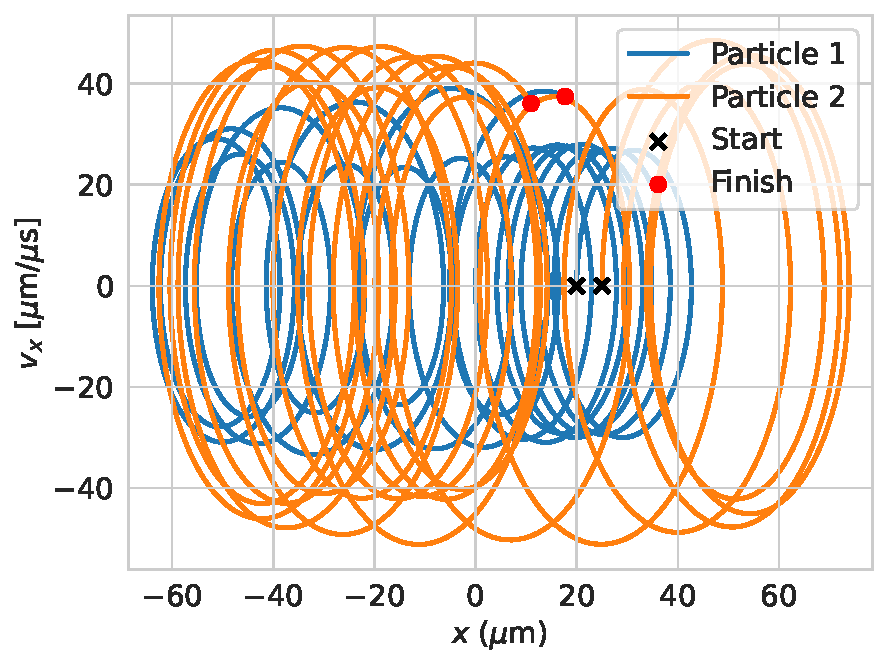
\includegraphics[width=.5\textwidth]{../figures/phase_space_x_interaction_RK4_N5000.pdf}
    \caption{The phase space $(x, v_x)$ of two particles with interaction for $N = 5000$.}
    \label{fig:RK4_2_x_phasespace_with_interaction_phasespace_xy}
\end{figure}
The two figures above show the trajectories of Particle 1 and Particle 2 in the $(x,v_x)$ plane.
Figure \ref{fig:RK4_2_x_phasespace_no_interaction_phasespace_xy} is a simulation disregarding particle interaction whilst
figure \ref{fig:RK4_2_x_phasespace_with_interaction_phasespace_xy} shows the trajectories with particle interaction. We
notice that the trajectories in figure \ref{fig:RK4_2_x_phasespace_no_interaction_phasespace_xy} are fairly repetitive whilst
figure \ref{fig:RK4_2_x_phasespace_with_interaction_phasespace_xy} shows more variations and different final points to figure
\ref{fig:RK4_2_x_phasespace_no_interaction_phasespace_xy}.

% Phase spaces z
\begin{figure}[H]
    \centering
    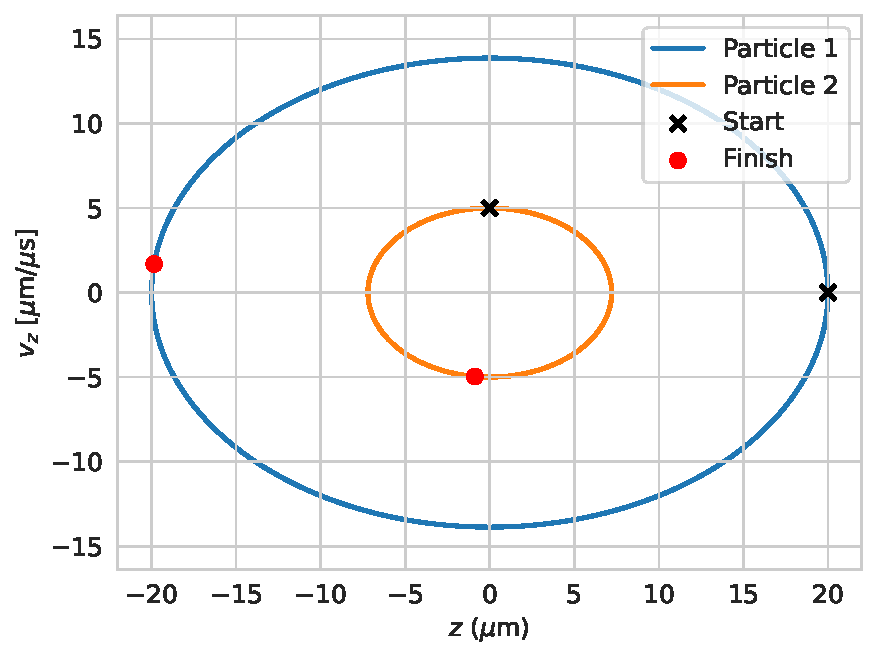
\includegraphics[width=.5\textwidth]{../figures/phase_space_z_RK4_N5000.pdf}
    \caption{The phase space $(z, v_z)$ of two particles without interaction for $N = 5000$.}
    \label{fig:K4_2_z_phasespace_no_interaction_phasespace_xy}
\end{figure}

\begin{figure}[H]
    \centering
    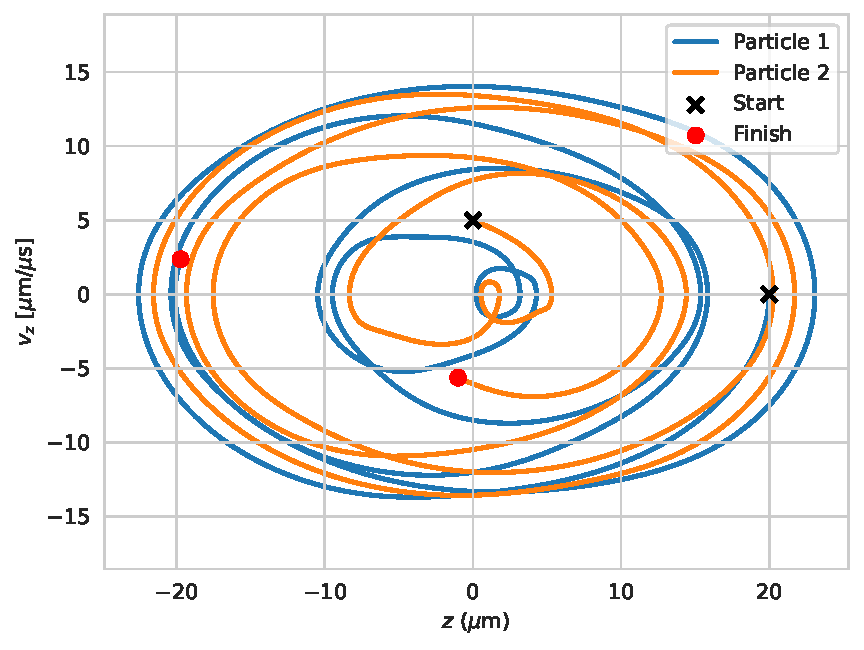
\includegraphics[width=.5\textwidth]{../figures/phase_space_z_interaction_RK4_N5000.pdf}
    \caption{The phase space $(z, v_z)$ of two particles with interaction for $N = 5000$.}
    \label{fig:K4_2_z_phasespace_with_interaction_phasespace_xy}
\end{figure}
Figures \ref{fig:K4_2_z_phasespace_no_interaction_phasespace_xy} and \ref{fig:K4_2_z_phasespace_with_interaction_phasespace_xy}
show the trajectories of Particle 1 and Particle 2 in the $(z,v_z)$ plane. In figure \ref{fig:K4_2_z_phasespace_no_interaction_phasespace_xy},
without particle interactions, we notice what seems to be repetitive trajectories similarly to figure
\ref{fig:RK4_2_x_phasespace_no_interaction_phasespace_xy}. Figure \ref{fig:K4_2_z_phasespace_with_interaction_phasespace_xy}
which includes particle interactions on the other hand displays more irregular trajectories similarly to figure \ref{fig:RK4_2_x_phasespace_with_interaction_phasespace_xy}.

%3D path plots
\begin{figure}[H]
    \centering
    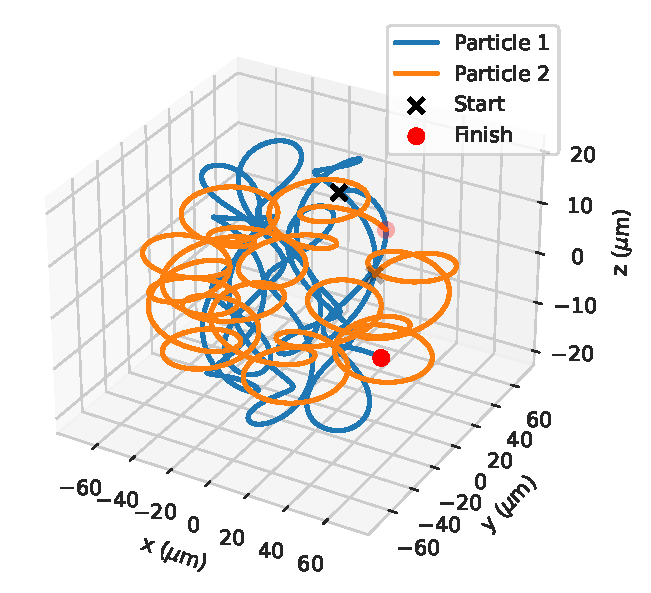
\includegraphics[width=.5\textwidth]{../figures/3D_2_particles_RK4_N5000.pdf}
    \caption{Shows a 3D representation of two particle paths without interaction for $N = 5000$.}
    \label{fig:3D_2_particles_no_interaction}
\end{figure}

\begin{figure}[H]
    \centering
    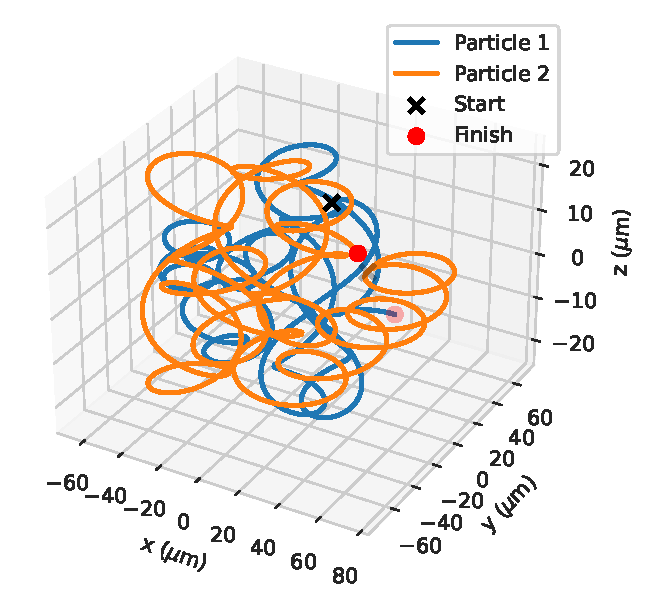
\includegraphics[width=.5\textwidth]{../figures/3D_2_particles_RK4_interaction_N5000.pdf}
    \caption{Shows a 3D representation of two particle paths with interaction for $N = 5000$.}
    \label{fig:3D_2_particles_with_interaction}
\end{figure}
Looking at the 3D-plots in figures \ref{fig:3D_2_particles_no_interaction} and \ref{fig:3D_2_particles_with_interaction}
it is difficult to follow the exact motion of the particles. Comparing figure \ref{fig:3D_2_particles_no_interaction}, without
particle interactions, to figure \ref{fig:3D_2_particles_with_interaction}, with interactions, one notices that the start positions
are identical, yet the finishing positions differ. Taking a close look it is also possible to see differences in the orange and blue
lines in the two figures.

Below in figure \ref{fig:relative_error_Euler_norm} and \ref{fig:relative_error_RK4_norm} we see plots of the relative error of our two numerical methods for different choices of $N$. We also see the belonging error convergence rate.
\begin{figure}[H]
    \centering
    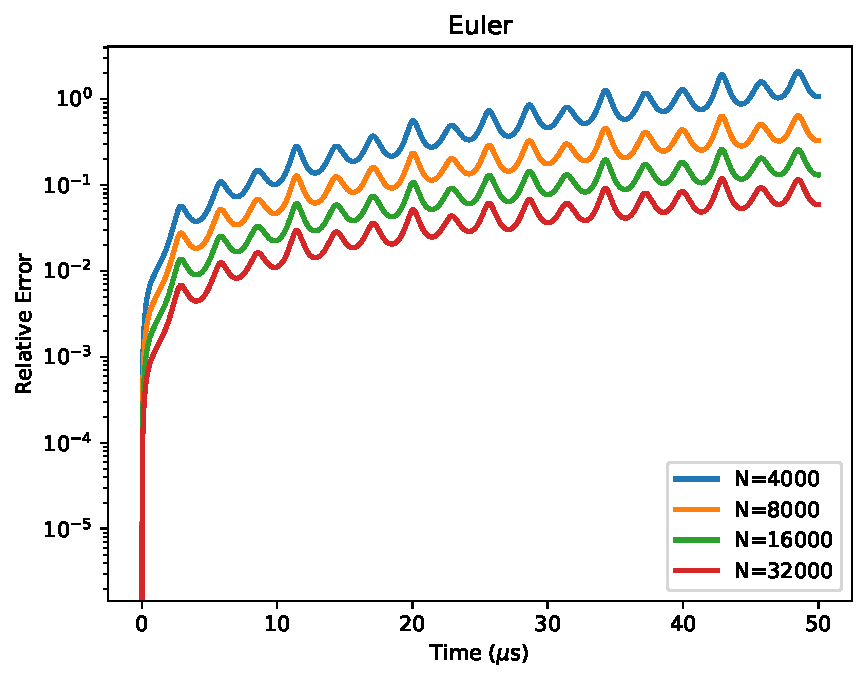
\includegraphics[width=.5\textwidth]{../figures/relative_error_Euler_norm.pdf}
    \caption{The plot shows the relative error for a single particle's motion over 50 $\mu s$ using the forward Euler approximation.
        The four different lines show results for different step sizes $h = 50/N \mu s$ }
    \label{fig:relative_error_Euler_norm}
\end{figure}

\begin{figure}[H]
    \centering
    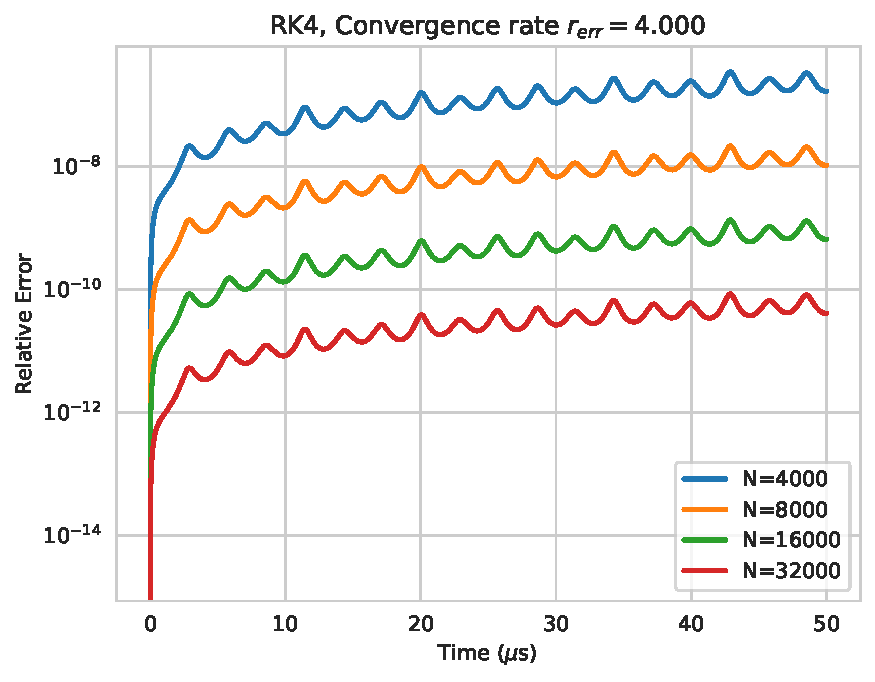
\includegraphics[width=.5\textwidth]{../figures/relative_error_RK4_norm.pdf}
    \caption{The plot shows the relative error for a single particle's motion over 50 $\mu s$ using the fourth order Runge-Kutta approximation.
        The four different lines show results for different step sizes $h = 50/N \mu s$ }
    \label{fig:relative_error_RK4_norm}
\end{figure}
We see that the error convergence rate of the RK4 method is 4 while the less accurate Euler has a convergence rate of 1.397. We notice that the logarithmic y-axis of the two figures are on different order and showing us the superiority of the RK4 method giving us more accurate results for $N=4000$ than Euler manages to do for $N=32000$. We also notice an oscillating nature of the relative error over time meaning that our methods perform worse for some particle positions than others.

Considering the case of a single particle to allow for a comparison to the analytic solution, figures \ref{fig:relative_error_Euler_norm}
and \ref{fig:relative_error_RK4_norm} display the relative error of the forward Euler method (figure \ref{fig:relative_error_Euler_norm})
and the RK4 method (figure \ref{fig:relative_error_RK4_norm}) for different step sizes $h = 50/N \mu s$. Noticeably for both
methods, the error decreases as the step size does too (increasing the number of points $N$). Comparing the two, one clearly
sees that the RK4 method is more precise than the forward Euler.

Under in figure \ref{fig:wide_freq_p_left_N_5000} we can see a wide frequency scan for three different amplitudes using a frequency step of $0.02$MHz.
Here we have again used $N=5000$ steps for the RK4 method
\begin{figure}[H]
    \centering
    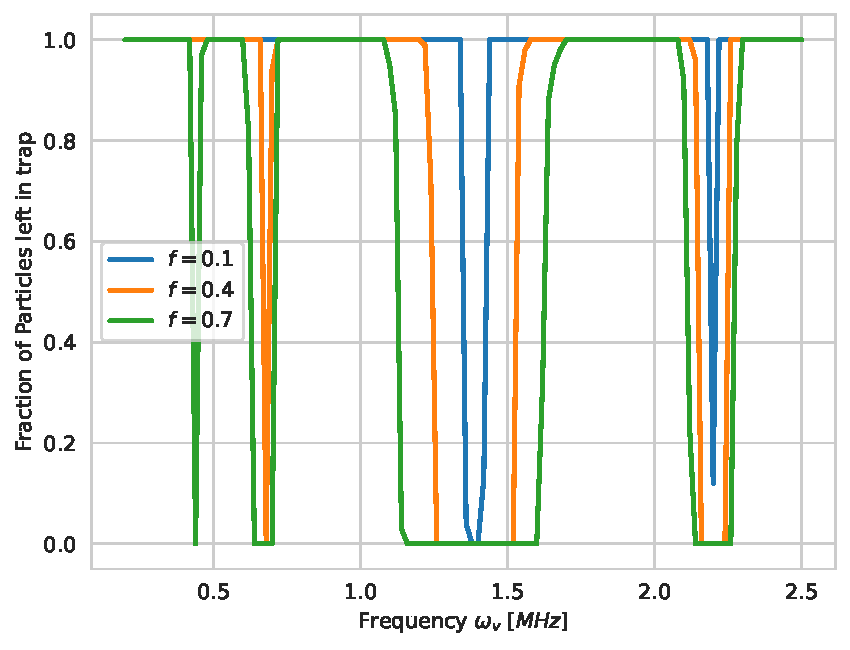
\includegraphics[width=.5\textwidth]{../figures/wide_freq_p_left_N_5000.pdf}
    \caption{The plot shows the fraction of particles that are left after 500 $\mu$s for angular frequencies $\omega_V \in (0.2,2.5)$MHz. Each color
            shows results for a different amplitude f. The simulation is for 100 random particles \textbf{without interactions}
            and $N = 5000$.}
    \label{fig:wide_freq_p_left_N_5000}
\end{figure}
We see 4 main frequency bands giving us a resonance in the motion of our particles. These are around a frequency of 0.45, 0.65, 1.4 and 2.2 MHz. We also see that the more narrow resonance bands needs a higher amplitude to throw the particles out of the Penningtrap. The most efficient ressonance frequencies are in other words the ones where even an amplitude of 0.1 is enough.

% zoomed without interaction
We continue with a frequency analysis and zoom in on frequencies in the interval [2.05, 2.35]MHz for a frequency step of 0.001MHz. This gives us figure \ref{fig:narrow_freq_p_left_N_5000_zoom}.
\begin{figure}[H]
    \centering
    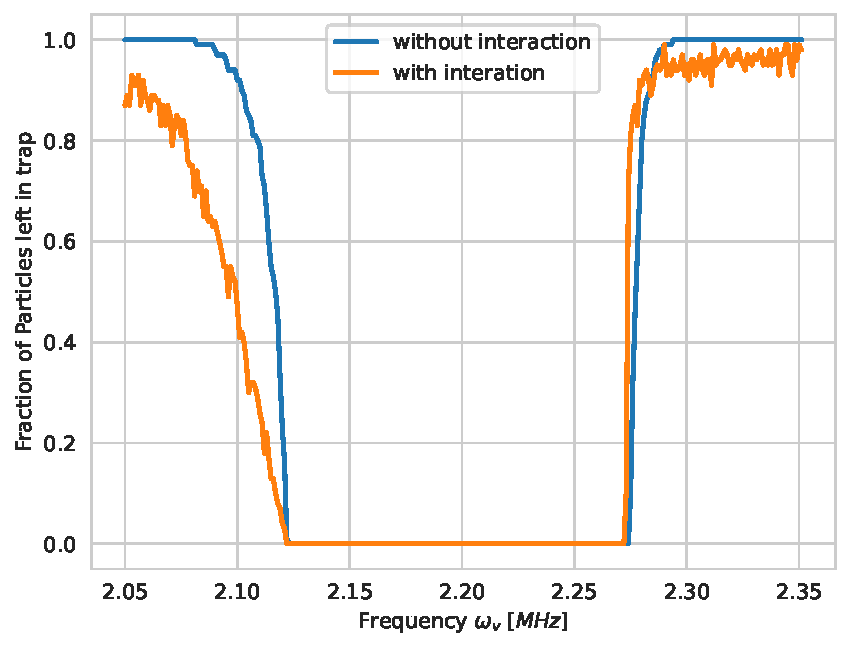
\includegraphics[width=.5\textwidth]{../figures/narrow_freq_p_left_N_5000_zoom.pdf}
    \caption{Shows the fraction of particles that are left after 500 $\mu$s for a zoomed in section of the frequency range
            is shown. The angular frequencies $\omega_V \in (2.05,2.35)$MHz are visible. Each color shows results for a
            different amplitude f. The simulation is for 100 random particles \textbf{without interactions} and $N = 5000$.}
    \label{fig:narrow_freq_p_left_N_5000_zoom}
\end{figure}
We see the same as we saw in figure \ref{fig:wide_freq_p_left_N_5000} just now with more details giving us a smoother plot.

By turning on particle interaction and looking at the same frequency spectrum we get the following plot in figure \ref{fig:narrow_freq_p_left_N_5000_interaction_zoom}.
%zoomed with interaction
\begin{figure}[H]
    \centering
    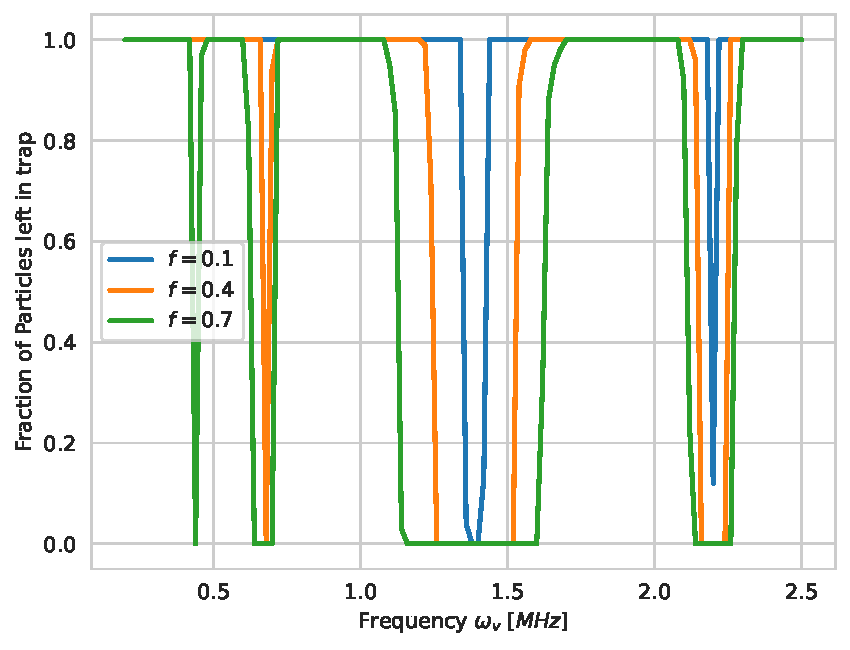
\includegraphics[width=.5\textwidth]{../figures/narrow_freq_p_left_N_5000_interaction_zoom.pdf}
    \caption{Shows the fraction of particles that are left after 500 $\mu$s for a zoomed in section of the frequency range
            is shown. The angular frequencies $\omega_V \in (2.05,2.35)$MHz are visible. Each color shows results for a
            different amplitude f. The simulation is for 100 random particles \textbf{with interactions} and $N = 5000$.}
    \label{fig:narrow_freq_p_left_N_5000_interaction_zoom}
\end{figure}
Here we see that the particle interactions clearly has an impact on how well the frequencies resonates with the motion of our particles. We see that some frequencies now resonates better than before and others that resonates worse. This is especially visible for frequencies around 2.05 and and 2.125 for $f=0.7$ which now have lower fractions left in the trap, and for frequencies of around 2.175 for $f=0.1$ that now have a higher fraction of particles left in the trap. We also see that most frequencies have lost at least some of the particles which compared to figure \ref{} where mostly all or no particles were lost.

% ===========================================
\section{Discussion}\label{sec:discussion}


Comparing figure \ref{fig:RK4_2_xy_no_interaction_xy} and \ref{fig:RK4_2_xy_with_interaction_xy} shows that the Coulomb force has a noticeable effect on
the particles motion since they repel each other. Here we look at only two particles interacting and the results with and without interactions are not extremely different,
but in a case of $n$ particles we would expect larger deviations between motion with and without interactions for increasing $n$.

Similarly, there are noticeable differences with and without interactions for the phase space $(x, v_x)$ in figure \ref{fig:RK4_2_x_phasespace_no_interaction_phasespace_xy}
and \ref{fig:RK4_2_x_phasespace_with_interaction_phasespace_xy} and the phase space $(z, v_z)$ in figure \ref{fig:K4_2_z_phasespace_no_interaction_phasespace_xy}
and \ref{fig:K4_2_z_phasespace_with_interaction_phasespace_xy}. From a physical point of view the results again seem reasonable. Specifically looking at
the phase space $(z, v_z)$, figure \ref{fig:K4_2_z_phasespace_no_interaction_phasespace_xy} without interaction shows a repetitive relation between velocity and position.
Figure \ref{fig:K4_2_z_phasespace_with_interaction_phasespace_xy} with interaction on the other hand shows a very different result as expected, since the particles
repel each other thereby affecting each other's velocities.

% The 3D-plots in figure \ref{fig:3D_2_particles_no_interaction}, without
% particle interactions, and figure \ref{fig:3D_2_particles_with_interaction}, with interactions allow us to see the full complexity of the particle motion.
% Already for two particles the paths are hard to follow.


The error analysis in figures \ref{fig:relative_error_Euler_norm} and \ref{fig:relative_error_RK4_norm} clearly shows that we gain
precision for smaller step sizes in the numerical simulations as expected. Furthermore, the fourth order Runge-Kutta method gives a better
approximation that the forward Euler method. This is again as expected since the local truncation error for Euler is $\mathcal{O}(h^2)$ and for RK4 is $\mathcal{O}(h^5)$.
The RK4 method thus deviating less from the analytical solution for small values of $h$.


%ERROR Discussion
We saw that the RK4 method was more accurate than Euler when comparing to the analytical solution for one particle. This makes sense when it comes to how the two numerical methods works. Euler uses the current position and velocity to step forward which for too large timesteps can result in the updated values deviating from the analytical solution. This means that the next forward step will use wrong values. Calculated values from the Euler method could then go towards infinity even in a atomic scale physics problem. This is avoided using RK4 where the forward stepping is determined by the slope at the beginning, midpoint and end of the interval. This way of stepping forward ensures a stability in our method as well as lowering our global error meaning that we for a too small $N$ only would see inaccurate values but not results going towards infinity.

% ===========================================
\section{Conclusion}\label{sec:conclusion}
\textit{In this section we state three things in a concise manner: what we have done, what we have found, and what should or could be done in the future.}

We have investigated the behavior of a Penning trap through numerical simulations, first exploring the basics of the simulation to then focus on
resonance phenomena. Our results show that
\onecolumngrid

%\bibliographystyle{apalike}
\bibliography{ref}


\end{document}
